\chapter{Ejercicios Resueltos}

\section{Ordenación elemental}
Escribí algoritmos para resolver cada uno de los siguientes problemas sobre un arreglo a de posiciones $1$ a $n$, utilizando do. Elegí en cada caso entre estos dos encabezados el que sea más adecuado:

\begin{codebox}{Ejercicio 1}
\begin{pascallike}
proc nombre (in/out a: array [1..n] of nat)
    ...
end proc
\end{pascallike}
\end{codebox}
\begin{codebox}{Ejercicio 1}
\begin{pascallike}
proc nombre (out a: array [1..n] of nat)
    ...
end proc
\end{pascallike}
\end{codebox}
\begin{itemize}
    \item[(a)] Inicializar cada componente del arreglo con el valor $0$.
    \item[(b)] Inicializar el arreglo con los primeros $n$ números naturales positivos.
    \item[(c)] Inicializar el arreglo con los primeros $n$ números naturales impares.
    \item[(d)] Incrementar las posiciones impares del arreglo y dejar intactas las posiciones pares.  
\end{itemize}

\begin{codebox}{Solución (a)}
\begin{pascallike}
proc inicializarConCero (out a: array [1..n] of nat)
    i := 1
    do i <= n -> 
    a[i] := 0
    i := i + 1
    od
end proc
\end{pascallike}
\end{codebox}
\begin{codebox}{Solución (b)}
\begin{pascallike}
proc inicializarConNaturales (out a: array [1..n] of nat)
    i := 1
    do i <= n -> 
    a[i] := i
    i := i + 1
    od
end proc
\end{pascallike}
\end{codebox}
\begin{codebox}{Solución (c)}
\begin{pascallike}
proc inicializarConImpares (out a: array [1..n] of nat)
    i := 1
    do i <= n -> 
    a[i] := 2 * i - 1
    i := i + 1
    od
end proc
\end{pascallike}
\end{codebox}
\begin{codebox}{Solución (d)}
\begin{pascallike}
proc incrementarImpares (in/out a: array [1..n] of nat)
    i := 1
    do i <= n -> 
    if i mod 2 = 1 then
        a[i] := a[i] + 1
    fi
    i := i + 1
    od
end proc
\end{pascallike}
\end{codebox}

\begin{center}
    \rule{\textwidth}{0.4pt}
\end{center}

Escribí un algoritmo que reciba un arreglo a de posiciones 1 a n y determine si el arreglo recibido está ordenado o no. Explicá en palabras \textbf{qué} hace el algoritmo. Explicá en palabras \textbf{cómo} lo hace.

\begin{codebox}{Solución}
\begin{pascallike}
fun estaOrdenado (a: array [1..n] of nat) ret r: bool
    r := true
    for i := 1 to n - 1 do
    if a[i] > a[i + 1] then
        r := false
    else
        skip
    fi
    od
end fun
\end{pascallike}
\end{codebox}

\begin{center}
    \rule{\textwidth}{0.4pt}
\end{center}
\newpage
Ordená los siguientes arreglos, utilizando el algoritmo de ordenación por selección visto en clase. Mostrá en cada paso de iteración cuál es el elemento seleccionado y cómo queda el arreglo después de cada intercambio.

\begin{itemize}
    \item[(a)] $[7, 1, 10, 3, 4, 9, 5]$
\end{itemize}

\begin{figure}[h]
    \centering
    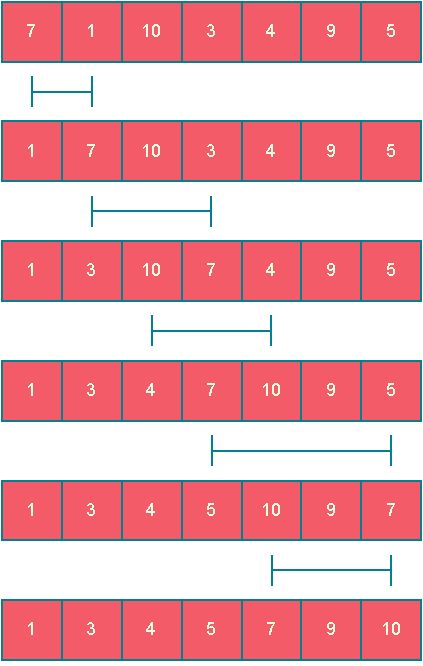
\includegraphics[scale=0.8]{estáticos/4a.pdf}
\end{figure}

\begin{center}
    \rule{\textwidth}{0.4pt}
\end{center}

Descifrá qué hacen los siguientes algoritmos, explicar cómo lo hacen y reescribirlos asignando nombres adecuados a todos los identificadores.

\begin{codebox}{Ejercicio 6 (a)}
\begin{pascallike}
proc p (in/out a: array [1..n] of T)
    var x: nat
    for i := n downto 2 do
    x := f(a,i)
    swap(a,i,x)
    od
end proc
\end{pascallike}
\end{codebox}

\begin{codebox}{Ejercicio 6 (b)}
\begin{pascallike}
fun f (a: array [1..n] of T, i: nat) ret x: nat
    x := 1
    for j := 2 to i do
    if a[j] > a[x] then
        x := j
    fi
    od
end fun
\end{pascallike}
\end{codebox}

\textbf{Algoritmo p:} El algoritmo recibe un arreglo de elementos de tipo T y lo ordena de manera descendente. Para ello, recorre el arreglo desde la última posición hasta la segunda, en cada iteración busca el elemento más grande en el subarreglo que va desde la primera posición hasta la posición actual y lo intercambia con el elemento en la posición actual.
Se podria escribir de la siguiente manera:

\begin{codebox}{Solución (a)}
\begin{pascallike}
proc ordenarDescendente (in/out a: array [1..n] of T)
    var posMax: nat
    for i := n downto 2 do
    posMax := buscarMaximo(a,i)
    swap(a,i,posMax)
    od
end proc
\end{pascallike}
\end{codebox}

\textbf{Función f:} La función recibe un arreglo de elementos de tipo T y un número natural $i$, y retorna la posición del elemento más grande en el subarreglo que va desde la primera posición hasta la posición $i$. Para ello, recorre el subarreglo desde la segunda posición hasta la posición $i$, en cada iteración compara el elemento actual con el elemento más grande encontrado hasta el momento y si el elemento actual es mayor, actualiza la posición del elemento más grande.
Se podria escribir de la siguiente manera:

\begin{codebox}{Solución (b)}
\begin{pascallike}
fun buscarMaximo (a: array [1..n] of T, i: nat) ret posMax: nat
    posMax := 1
    for j := 2 to i do
    if a[j] > a[posMax] then
        posMax := j
    fi
    od
end fun
\end{pascallike}
\end{codebox}

\section{Ordenación avanzada}

\begin{itemize}
    \item[a)] Escribí el procedimiento "\texttt{intercalar\_cada}" que recibe un arreglo $a : array[1..2^n] of int$ y un número natural $i : nat$; e intercala el segmento $a[1, 2^i]$ con $a[2^i + 1, 2 * 2^i]$, el segmento $a[2 * 2^i + 1, 3 * 2^i]$ con $a[3 * 2^i + 1, 4 * 2^i]$, etc. Cada uno de dichos segmentos se asumen ordenados. Por ejemplo, si el arreglo contiene los valores $3, 7, 1, 6, 1, 5, 3, 4$ y se lo invoca con con $i = 1$ el algoritmo deberá devolver el arreglo $1, 3, 6, 7, 1, 3, 4, 5$. Si se lo vuelve a invocar con este nuevo arreglo y con $i = 2$, devolverá $1, 1, 3, 3, 4, 5, 6, 7$ que ya está completamente ordenado. El algoritmo asume que cada uno de estos segmentos está ordenado, y puede utilizar el procedimiento de intercalación dado en clase
    \item[b)] Utilizar el algoritmo "\texttt{intercalar\_cada}" para escribir una versión iterativa del algoritmo de ordenación por intercalación. La idea es que en vez de utilizar recursión, invoca al algoritmo del inciso anterior sucesivamente con $i = 0, 1, 2, 3,$ etc.
\end{itemize}

Primero para definir el procedimiento, va a recibir un arreglo \texttt{a : array[1..$2^n$] of int} y un número natural $i : nat$:

\begin{codebox}{Estructura}
\begin{pascallike}
proc intercalar_cada(in/out a: array[1..$2^n$] of Int, in i: nat)
...
end proc
\end{pascallike}
\end{codebox}
para poder intercalar el arreglo, se va a tener que llamar a la función \texttt{merge}, que toma un arreglo, y 3 posiciones \texttt{lft}, \texttt{mid}, \texttt{rgt}. Entonces hay que definirlas:

\begin{codebox}{Inicialización de variables}
\begin{pascallike}
proc intercalar_cada(in/out a: array[1..$2^n$] of Int, in i: nat)
    var lft, rgt, mid: nat
    ...
end proc
\end{pascallike}
\end{codebox}
Se deberia agregar una variable natural para recorrer cada segmento del arreglo

\begin{codebox}{Inicialización de variables}
\begin{pascallike}
proc intercalar_cada(in/out a: array[1..$2^n$] of Int, in i: nat)
    var lft, rgt, mid: nat {-Variables para llamar a merge-}
    var k: nat {-Variable para recorrer el arreglo-}
    ...
end proc
\end{pascallike}
\end{codebox}
La idea principal es realizar la intercalación de segmentos del arreglo según el valor proporcionado \texttt{i}, cada segmento tiene un tamaño de $2^i$ elementos. Para ello se debe hacer un ciclo while que calcule cada uno de los índices para llamar a la función de intercalación.

\begin{codebox}{Ciclo while}
\begin{pascallike}
proc intercalar_cada(in/out a: array[1..$2^n$] of Int, in i: nat)
    var lft, rgt, mid: nat {-Variables para llamar a merge-}
    var k: nat {-Variable para recorrer el arreglo-}
    while k $\leq$ $2^n$ do
    lft := ... {-Indice inicial del primer segmento-}
    mid := ... {-Indice final del primer segmento-}
    rgt := ... {-Indice final del segundo segmento-}
    merge(a,lft,mid,rgt) {-Llamada a la funcion para intercalar-}
    k := ...
    do
end proc
\end{pascallike}
\end{codebox}
El índice lft será primero $1$, siguiendo la estructura de los segmentos, deberia tomar el valor de $k * 2^i + 1$, luego el medio es $(j+1) * 2^i$ y el final es $(j+2) * 2^i$.
\begin{codebox}{Procedimiento completo}
\begin{pascallike}
proc intercalar_cada(in/out a: array[1..$2^n$] of Int, in i: nat)
    var lft, rgt, mid: nat {-Variables para llamar a merge-}
    var k: nat {-Variable para recorrer el arreglo-}
    while k $\leq$ $2^n$ do
    lft := k * $2^i$ + 1 {-Indice inicial del primer segmento-}
    mid := (k+1) * $2^i$ {-Indice final del primer segmento-}
    rgt := (k+2) * $2^i$ {-Indice final del segundo segmento-}
    merge(a,lft,mid,rgt) {-Llamada a la funcion para intercalar-}
    k := k+2
    do
end proc
\end{pascallike}
\end{codebox}
\begin{codebox}{Solución}
\begin{pascallike}
proc intercalar_cada_iter (in/out array[1..$2^n$] of int)
    for i := 0 to n-1 do
    intercalar_cada(a,i)
    od
end proc
\end{pascallike}
\end{codebox}

\begin{center}
    \rule{\textwidth}{0.4pt}
\end{center}

Escribí un algoritmo que dado un arreglo \texttt{a : array[1..n] of int} y un número natural $k \leq n$ devuelve el elemento de \texttt{a} que quedaría en la celda \texttt{a[k]} si a estuviera ordenado. Está permitido realizar intercambios en \texttt{a}, pero no ordenarlo totalmente. La idea es explotar el hecho de que el procedimiento partition del quick sort deja al pivot en su lugar correcto.

\begin{codebox}{Algoritmo}
\begin{pascallike}
fun encontrarElemento(a: array[1..n] of int, k: nat): ret r : int
    var lft, rgt, ppiv: nat

    lft := 1
    rgt := n

    do lft < rgt -->
        partition(a, lft, rgt, ppiv)

        if ppiv = k -->
            r := a[ppiv]
        [] ppiv < k -->
            lft := ppiv + 1
        [] -->
            rgt := ppiv - 1
        fi
    od

    r := a[k]
end proc
\end{pascallike}
\end{codebox}

\begin{center}
    \rule{\textwidth}{0.4pt}
\end{center}

El procedimiento \texttt{partition} que se dio en clase separa un fragmento de arreglo principalmente en dos segmentos: menores o iguales al pivot por un lado y mayores o iguales al pivot por el otro. Modificá ese algoritmo para que separe en tres segmentos: los menores al pivot, los iguales al pivot y los mayores al pivot. En vez de devolver solamente la variable \texttt{pivot}, deberá devolver \texttt{pivot izq} y \texttt{pivot} der que informan al algoritmo \texttt{quick\_sort\_rec} las posiciones inicial y final del segmento de repeticiones del \texttt{pivot}. Modificá el algoritmo \texttt{quick\_sort\_rec} para adecuarlo al nuevo procedimiento \texttt{partition}.

\textbf{Procedimiento \texttt{partition} modificado:}

\begin{codebox}{Partition modificado}
\begin{pascallike}
proc partition(in/out a: array[1..n] of T, in lft, rgt: nat, 
out pivotIzq, pivotDer: nat)
    var i, j, pivotPos: nat
    {-pivotPos rastrea la posicion actual del pivote-}
    pivotPos := lft
    i := lft + 1
    j := rgt

    do i <= j -->
        {-Casos para manejar elementos menores, mayores e iguales al pivote-}
        if a[i] < a[pivotPos] -->
            i := i + 1
        [] a[j] > a[pivotPos] -->
            j := j - 1
        [] a[i] > a[pivotPos] -->
            swap(a, i, j)
        {-Caso para manejar repeticiones del pivote-}
        [] -->
            swap(a, i, pivotPos)
            pivotPos := i
            i := i + 1
            j := j - 1
        fi
    od
    {-pivotIzq es la posicion inicial del segmento de repeticiones del pivote-}
    pivotIzq := lft
    {-pivotDer es la posicion final del segmento de repeticiones del pivote-}
    pivotDer := j
    {-Mover todas las repeticiones del pivote a posiciones contiguas despues 
    de pivotIzq-}
    do j < rgt -->
        swap(a, j + 1, rgt)
        j := j + 1
    od
end proc

proc quick_sort_rec(in/out a: array[1..n] of T, in lft, rgt: nat)
    var pivotIzq, pivotDer: nat

    if lft < rgt -->
        partition(a, lft, rgt, pivotIzq, pivotDer)
        quick_sort_rec(a, lft, pivotIzq - 1)
        quick_sort_rec(a, pivotDer + 1, rgt)
    fi
end proc
\end{pascallike}
\end{codebox}

\section{Recurrencia Divide y Vencerás}

Calculá el orden de complejidad de los siguientes algoritmos:

\begin{codebox}{(a)}
\begin{pascallike}
proc f1(in n : nat)
    if n $\leq$ 1 then skip
    else
        for i := 1 to 8 do 
            f1(n div 2) 
        od
        for i := 1 to $n^3$ do 
            t := 1 
        od
    fi
end proc
\end{pascallike}
\end{codebox}

\begin{codebox}{(b)}
\begin{pascallike}
proc f2(in n : nat)
    for i := 1 to n do
        for j := 1 to i do 
            t := 1 
        od
    od
    if n > 0 then
        for i := 1 to 4 do 
            f2(n div 2) 
        od
    fi
end proc
\end{pascallike}
\end{codebox}

\textbf{Solución (a)}
En este caso notar que:
\begin{itemize}
    \item Tamaño de la entrada: $n$,
    \item Operación a contar: $t := 1$.
\end{itemize}
Entonces, se puede definir una funcion $r(n)$, que representará la cantidad de asignaciones a la variable $t$ que ocurren al llamar a la función $f1$ con el dato de entrada $n$.

Podemos observar que la función $f1$ esta dividida en dos casos, si $n \leq 1$ entonces no se realiza ninguna asignación a la variable $t$, por lo que $r(n) = 0$.
\begin{equation*}
    r(n) = 
    \begin{cases}
        0 & \text{si } n \leq 1 \\
        ... & \text{en caso contrario}
    \end{cases}
\end{equation*}
Como hay dos ciclos for en una secuencia, se puede analizar cada uno por separado y sumarlos, por ahora los puedo expresar como sumatoria:
\begin{equation*}
    r(n) = 
    \begin{cases}
        0 & \text{si } n \leq 1 \\
        \sum_{i=1}^{8} ... + \sum_{i=1}^{n^3} ... & \text{en caso contrario}
    \end{cases}
\end{equation*}
En el primer for, queremos contar la cantidad de asignaciones que se realizan al llamar a la función $f1$ con el dato de entrada $n/2$, por lo que se puede expresar como:
\begin{equation*}
    r(n) = 
    \begin{cases}
        0 & \text{si } n \leq 1 \\
        \sum_{i=1}^{8} r(n/2) + \sum_{i=1}^{n^3} ... & \text{en caso contrario}
    \end{cases}
\end{equation*}
En el segundo for, se realiza una asignación a la variable $t$ por cada iteración, por lo que se puede expresar como:
\begin{equation*}
    r(n) = 
    \begin{cases}
        0 & \text{si } n \leq 1 \\
        \sum_{i=1}^{8} r(n/2) + \sum_{i=1}^{n^3} 1 & \text{en caso contrario}
    \end{cases}
\end{equation*}
Resolviendo las sumatorias, se obtiene:
\begin{equation*}
    r(n) = 
    \begin{cases}
        0 & \text{si } n \leq 1 \\
        8 \cdot r(n/2) + n^3 & \text{en caso contrario}
    \end{cases}
\end{equation*}
Por lo que se puede observar que:
\begin{itemize}
    \item $a = 8$,
    \item $b = 2$,
    \item $g(n) = n^3$.
\end{itemize}
Como $a = 8 = 2^3 = b^3$, se puede decir que el orden de complejidad es $O(n^3 \log n)$.

\textbf{Solución (b)}
En este caso notar que:
\begin{itemize}
    \item Tamaño de la entrada: $n$,
    \item Operación a contar: $t := 1$.
\end{itemize}
Entonces, se puede definir una funcion $r(n)$, que representará la cantidad de asignaciones a la variable $t$ que ocurren al llamar a la función $f2$ con el dato de entrada $n$.

En este caso la función $f2$ está dividida en $n$ casos (cada uno representado por el valor de $i$):
\begin{equation*}
    r(n) = 
    \begin{cases}
        \sum_{i=1}^{n} \sum_{j=1}^{i} 1 & \text{casos simples }  \\
        ... & \text{en caso contrario}
    \end{cases}
\end{equation*}
En el for dentro del if, se realiza una llamada recursiva a la función $f2$ con el dato de entrada $n/2$, por lo que se puede expresar como:
\begin{equation*}
    r(n) = 
    \begin{cases}
        \sum_{i=1}^{n} \sum_{j=1}^{i} 1 & \text{casos simples }  \\
        \sum_{i=1}^{n} \sum_{j=1}^{i} 1 +  \sum_{i=1}^{4} r(n/2) & \text{en caso contrario}
    \end{cases}
\end{equation*}
Resolviendo las sumatorias, se obtiene:
\begin{equation*}
    r(n) = 
    \begin{cases}
        \sum_{i=1}^{n} i & \text{casos simples }  \\
        \sum_{i=1}^{n} i +  \sum_{i=1}^{4} r(n/2) & \text{en caso contrario}
    \end{cases}
\end{equation*}
\begin{equation*}
    r(n) = 
    \begin{cases}
        \frac{n\cdot (n+1)}{2} & \text{casos simples }  \\
        \frac{n\cdot (n+1)}{2} + 4 \cdot r(n/2) & \text{en caso contrario}
    \end{cases}
\end{equation*}

Por lo que se puede observar que:
\begin{itemize}
    \item $a = 4$,
    \item $b = 2$,
    \item $g(n) = \frac{n\cdot (n+1)}{2}$.
\end{itemize}
Como $a = 4 = 2^2 = b^2$, se puede decir que el orden de complejidad es $O(n^2 \log n)$.

\begin{center}
    \rule{\textwidth}{0.4pt}
\end{center}

Dado un arreglo \texttt{a : array[1..n] of nat} se define una cima de $a$ como un valor $k$ en el intervalo $1, . . . ,n$ tal que $a[1..k]$ está ordenado crecientemente y $a[k..n]$ está ordenado decrecientemente.
\begin{itemize}
    \item[(a)] Escribá un algoritmo que determine si un arreglo dado tiene cima.
    \item[(b)] Escribí un algoritmo que encuentre la cima de un arreglo dado (asumiendo que efectivamente tiene una cima) utilizando una búsqueda secuencial, desde el comienzo del arreglo hacia el final. 
    \item[(c)] Escribí un algoritmo que resuelva el mismo problema del inciso anterior utilizando la idea de \texttt{búsqueda binaria}.
    \item[(d)] Calculá y compará el orden de complejidad de ambos algoritmos.
\end{itemize}

Para determinar si un arreglo tiene cima, se puede recorrer el arreglo y buscar el máximo que va a ser el probable punto cima.

\begin{codebox}{Estructura}
\begin{pascallike}
fun tieneCima (a : array[1..n] of nat) ret r : bool
    r := false
    var tempos : nat
    {-Busco la posible cima y lo guardo en tempos-}
    for i := 2 to n do
        if a[i-1] < a[i] then
            tempos := i
            r := true
        fi
    od
    ...
end fun
\end{pascallike}
\end{codebox}

Luego de encontrar un elemento, habria que verificar si el resto del arreglo cumple con la condición de cima.

\begin{codebox}{Solución final}
\begin{pascallike}
fun tieneCima (a : array[1..n] of nat) ret r : bool
    r := false
    var tempos : nat
    {-Busco la posible cima y lo guardo en tempos-}
    for i := 2 to n do
        if a[i-1] < a[i] then
            tempos := i
            r := true
        fi
    od
    {-Si hay alguna posible cima, verifico que el resto arreglo cumpla-}
    for i := 1 to tempos do
        if a[i] < a[i+1] then
            r := false
        fi
    od
    for i := tempos to n do
        if a[i] > a[i+1] then
            r := false
        fi
    od
end fun
\end{pascallike}
\end{codebox}

Para encontrar la cima y devolverla, el algoritmo es el mismo que el anterior con la diferencia de que en vez de devolver el valor de r, devuelvo el valor del arreglo en la posición tempos (y la verificación de si hay cima o no se puede omitir ya que se asume que hay cima).

\begin{codebox}{Solución final}
\begin{pascallike}
fun cima (a : array[1..n] of nat) ret c : nat
    var tempos : nat
    {-Busco la cima y lo guardo en tempos-}
    for i := 2 to n do
        if a[i-1] < a[i] then
            tempos := i
        fi
    od
    c := a[tempos]
end fun
\end{pascallike}
\end{codebox}

Para encontrar la cima y devolverla, se puede utilizar la idea de búsqueda binaria. Se puede buscar el punto cima de la siguiente manera:

\begin{itemize}
    \item Se toma el punto medio del arreglo y se compara con el siguiente elemento.
    \item Si el punto medio es menor al siguiente elemento, entonces la cima se encuentra en la mitad derecha del arreglo.
    \item Si el punto medio es mayor al siguiente elemento, entonces la cima se encuentra en la mitad izquierda del arreglo.
\end{itemize}

\begin{codebox}{Solución}
\begin{pascallike}
fun busqueda_binaria_rec (a : array[1..n] of nat, lft, rgt: nat) ret i : nat
var mid : nat
if lft < rgt then
    i := 0
else
    mid := (lft + rgt) div 2
    if a[mid-1] $\geq$ a[mid] $\wedge$ a[mid+1] $\geq$ a[mid] then
        i := busqueda_binaria_rec(a, lft, mid-1)
    fi
    if a[mid-1] $\leq$ a[mid] $\wedge$ a[mid+1] $\leq$ a[mid] then
        i := mid
    fi
    if a[mid-1] $\leq$ a[mid] $\wedge$ a[mid+1] $\geq$ a[mid] then
        i := busqueda_binaria_rec(a, mid+1, rgt)
    fi
fi
end fun

fun cima (a : array[1..n] of nat) ret c : nat
    c := busqueda_binaria_rec(a, 2, n-1)
end fun
\end{pascallike}
\end{codebox}

\textbf{Solución (d)}
Para el algoritmo de búsqueda secuencial, se puede observar que el peor caso es cuando la cima se encuentra en la última posición del arreglo, por lo que se recorre todo el arreglo. Por lo que el orden de complejidad es $O(n)$.

Para el algoritmo de búsqueda binaria, se puede observar que el peor caso es cuando la cima se encuentra en la mitad del arreglo, por lo que se divide el arreglo en dos partes y se busca en una de ellas. Por lo que el orden de complejidad es $O(\log n)$.

\newpage
\section{Tipos de datos concretos}

Escribir un algoritmo que dada una matriz \texttt{a: array[1..n,1..m] of int} calcule el elemento mínimo. Escribir otro algoritmo que devuelva un arreglo \texttt{array[1..n]} con el mínimo de cada fila de la matriz \texttt{a}.

\begin{codebox}{Ejercicio 1.1}
\begin{pascallike}
fun min_elem_array(a : array[1..n,1..m] of int) ret min_elem int
    min_elem := a[1][1];
    for fil:= 1 to n do
        for col:= 1 to m do
            if a[fil][col] < min_elem then
                min_elem := a[col][fil];
            fi
        od
    od
end fun
\end{pascallike}
\end{codebox}

\begin{codebox}{Ejercicio 1.2}
\begin{pascallike}
fun array_of_mins(a: array[1..n,1..m] of int) ret array_min array[1..n] of int
    for fil:= 1 to n do
        array_min[fil] := min_elem_array(a[fil, 1..m])
    od
end fun
\end{pascallike}
\end{codebox}

\begin{center}
    \rule{\textwidth}{0.4pt}
\end{center}

Dados los tipos enumerados

\begin{codebox}{mes}
\begin{pascallike}
type mes = enumerate
            enero
            febrero
            ...
            diciembre
           end enumerate
\end{pascallike}
\end{codebox}

\begin{codebox}{clima}
\begin{pascallike}
type clima = enumerate
                Temp
                TempMax
                TempMin
                Pres
                Hum
                Prec
             end enumerate
\end{pascallike}
\end{codebox}

El arreglo \texttt{med:array[1980..2016,enero..diciembre,1..28,Temp..Prec] of nat} es un arreglo multidimensional que contiene todas las mediciones estadísticas del clima para la ciudad de Córdoba desde el 1/1/1980 hasta el 28/12/2016. Por ejemplo, \texttt{med[2014,febrero,3,Pres]} indica la presión atmosférica que se registró el día 3 de febrero de 2014. Todas las mediciones están expresadas con números enteros. Por simplicidad asumiremos que todos los meses tienen 28 días.

\begin{itemize}
    \item[(a)] Dar un algoritmo que obtenga la menor temperatura mínima (TempMin) histórica registrada en la ciudad de Córdoba según los datos del arreglo.
    \item[(b)] Dar un algoritmo que devuelva un arreglo que registre para cada año entre 1980 y 2016 la mayor temperatura máxima (TempMax) registrada durante ese año.
    \item[(c)] Dar un algoritmo que devuelva un arreglo que registre para cada año entre 1980 y 2016 el mes de ese año en que se registró la mayor cantidad mensual de precipitaciones (Prec).
    \item[(d)] Dar un algoritmo que utilice el arreglo devuelto en el inciso anterior (además de med) para obtener el año en que ese máximo mensual de precipitaciones fue mínimo (comparado con los de otros años).
    \item[(e)]  Dar un algoritmo que obtenga el mismo resultado sin utilizar el del inciso (c)
\end{itemize}

\begin{codebox}{Ejercicio 2.a}
\begin{pascallike}
fun min_tempMin (a:array[1980..2016,enero..diciembre,1..28,Temp..Prec] of nat) 
ret min_temp int
    temp_min:= a[1980,enero,1,TempMin]
    for a:= 1980 to 2016 do
        for m:= enero to diciembre do
            for d:= 1 to 28 do
                if (a[a,m,d,TempMin] < temp_min) then
                    temp_min:= a[a,m,d,TempMin]
                fi 
            od
        od
    od
end fun
\end{pascallike}
\end{codebox}

\begin{codebox}{Ejercicio 2.b}
\begin{pascallike}
fun temp_max_a(a:array[1980..2016,enero..diciembre,1..28,Temp..Prec] of nat)
ret res:array[1980..2016] of int
    var max_a_temp: int
    for a:= 1980 to 2016 do
        max_a_temp:= a[a,1,1,TempMax]
        for mes:= enero to diciembre do
            for dia:= 1 to 28 do
            if(max_a_temp < a[a,m,d,TempMax]) then
                res[a]:= a[a,m,d,TempMax]
            fi
            od
        od
    od
end fun
\end{pascallike}
\end{codebox}

\begin{codebox}{Ejercicio 2.c}
\begin{pascallike}
fun mes_max_prec(a:array[1980..2016,enero..diciembre,1..28,Temp..Prec] of nat)
ret res:array[1980..2016] of mes
    var max_mes : mes
    var max_mes_prec, mas_prec : nat

    for a := 1980 to 2016 do
        {-calcular max_mes para cada anio-}
        max_mes_prec := 0
        for mes := enero to diciembre do
            {-calcular la suma prec_mes para cada mes-}
            prec_mes := 0
            for dia := 1 to 28 do
                prec_mes := prec_mes + a[a,mes,dia,Prec]
            od
            if prec_mes >= max_mes_prec then
                max_mes_prec := prec_mes
                max_mes := mes
            fi
        od
        res[a] := max_mes
    od
end fun
\end{pascallike}
\end{codebox}

\begin{codebox}{Ejercicio 2.d}
\begin{pascallike}
fun min_prec_mes(a:array[1980..2016,enero..diciembre,1..28,Temp..Prec] of nat)
ret res_a: int
    var meses: array[1980..2016] of string
    var prec_meses: array[1980..2016] of string
    meses:= mes_may_prec(a)
    for mes := enero to diciembre do
            {-calcular la suma prec_mes para cada mes-}
            prec_mes := 0
            for dia := 1 to 28 do
                prec_mes := prec_mes + a[a,mes,dia,Prec]
            od
            if prec_mes >= max_mes_prec then
                max_mes_prec := prec_mes
                max_mes := mes
            fi
        od
    var min_prec: int
    min_prec:= prec_meses[1980]
    res_a:= 1980
    for a:= 1981 to 2016 do
        if(prec_meses[a] < min_prec) then
            min_prec:= prec_meses[a]
            res_a:= a
        fi
    od
end fun
\end{pascallike}
\end{codebox}

\begin{codebox}{Ejercicio 2.e}
\begin{pascallike}
fun min_prec_mes_2(a:array[1980..2016,enero..diciembre,1..28,Temp..Prec] of nat) 
        ret res:array[1980..2016] of int
    {- primer algoritmo-}
    var res_tmp, prec_mes: int
    for an:= 1980 to 2016 do
        res_tmp:= 0
        for mes:= enero to diciembre do
            prec_mes:= 0
            for dia:= 1 to 28 do
            prec_mes:= prec_mes + a[an,mes,dia,Prec]
            od
            if(res_tmp < prec_mes) then
            res_parte1[an]:= mes
            res_tmp:= prec_mes
        od
    od
    {-segundo algoritmo-}
    var meses: array[1980..2016] of string
    var prec_meses: array[1980..2016] of string
    for an:= 1980 to 2016 do
        for dia:= 1 to 28 do
            prec_mes:= prec_mes + a[an,res_parte1[n],dia,Prec]
        od
        prec_meses[an]:= prec_mes
    od
    var min_prec: int
    min_prec:= prec_meses[1980]
    res_an:= 1980
    for an:= 1981 to 2016 do
        if(prec_meses[an] < min_prec) then
            min_prec:= prec_meses[an]
            res_an:= an
        fi
    od
end proc
\end{pascallike}
\end{codebox}

\begin{center}
    \rule{\textwidth}{0.4pt}
\end{center}

Dados dos arreglos \texttt{a, b : array[1..n] of nat} se dice que a es \texttt{“lexicográficamente menor”} que b si existe $k \in {1 . . . n}$ tal que \texttt{a[k] < b[k]}, y para todo $i \in {1 . . . k - 1}$ se cumple \texttt{a[i] = b[i]}. En otras palabras, si en la primera posición en que $a$ y $b$ difierente, el valor de $a$ es menor que el de $b$. También se dice que $a$ es \textit{“lexicográficamente menor o igual”} a $b$ si $a$ es lexicográficamente menor que b o a es igual a $b$.

\begin{itemize}
    \item[(a)] Escribir un algoritmo lex less que recibe ambos arreglos y determina si a es lexicográficamente menor que b.
    \item[(b)] Escribir un algoritmo lex less or equal que recibe ambos arreglos y determina si a es lexicográficamente menor o igual a b. 
    \item[(c)] Dado el tipo enumerado
\begin{codebox}{tipo}
\begin{pascallike}
type ord = enumerate
             igual
             menor
             mayor
           end enumerate
\end{pascallike}
\end{codebox}
Escribir un algoritmo lex compare que recibe ambos arreglos y devuelve valores en el tipo ord. ¿Cuál es el interés de escribir este algoritmo?
\end{itemize}

\begin{codebox}{Ejercicio 5.a}
\begin{pascallike}
fun lex_less(a,b : array[1..n] of nat) ret res: bool
    res := false
    if a[1] < b[1] then
        res := true
    else
        for i:= 1 to n do
            if a[i] < b[i] then
                res := true
                break
            fi
        od
    fi
end fun
\end{pascallike}
\end{codebox}
\textbf{Inicialización:} Se declara una variable res y se inicializa a false. Esta variable almacenará el resultado final que indica si a es lexicográficamente menor que b.
\textbf{Comparando los primeros elementos:} 
\begin{itemize}
    \item El código verifica si el primer elemento de a (indicado por a[1]) es menor que el primer elemento de b (indicado por b[1]).
    \item Si lo es, entonces res se establece inmediatamente a true. Esto se debe a que en la comparación lexicográfica, el arreglo con el primer elemento más pequeño se considera menor.
\end{itemize}
\textbf{Iterando por los arreglos:} 
\begin{itemize}
    \item Si los primeros elementos no son diferentes, el código entra en un ciclo que itera desde el índice 1 hasta n (la longitud de los arreglos).
    \item Dentro del ciclo, compara los elementos en el índice actual (i) de ambos arreglos (a[i] y b[i]).
    \begin{itemize}
        \item Si se encuentra que un elemento en a es menor que el elemento correspondiente en b, entonces res se establece en true y el ciclo se detiene (break) usando la instrucción break. Esto se debe a que una vez que se encuentra una diferencia donde a tiene un elemento más pequeño que b, sabemos que a es lexicográficamente menor y no hay necesidad de seguir iterando.
        \item Si se encuentra que un elemento en a es mayor que el elemento correspondiente en b, el ciclo termina inmediatamente devolviendo false. Esto se debe a que si a tiene un elemento mayor en cualquier punto, no puede ser lexicográficamente menor que b.
    \end{itemize}
\end{itemize}
\textbf{Resultado:} Una vez que el ciclo termina de iterar por todos los elementos, si no se encuentra ninguna diferencia (a y b tienen los mismos elementos en todo), entonces res seguirá siendo false.

\begin{codebox}{Ejercicio 5.b}
\begin{pascallike}
fun lex_less(a,b : array[1..n] of nat) ret res: bool
    res := false
    if a[1] < b[1] then
        res := true
    else
        for i:= 1 to n do
            if a[i] < b[i] then
                res := true
                break
            fi
        od
        if not res then
        res := true
        fi
    fi
end fun
\end{pascallike}
\end{codebox}

\begin{codebox}{Ejercicio 5.c}
\begin{pascallike}
fun lex_less(a,b : array[1..n] of nat) ret res: ord
    var comp: ord
    res := igual
    if a[1] < b[1] then
    comp := menor
    else if a[1] > b[1] then
    comp := mayor
    else
    for i:= 2 to n do
        if a[i] < b[i] then
            comp := menor
            break
        fi
        if comp = mayor then
            break
        fi
    od
    fi
    res := comp
end fun
\end{pascallike}
\end{codebox}

\textbf{Comparación de primeros elementos:} Se compara el primer elemento de a y b. Si a[1] < b[1], se establece comp en menor. Si a[1] > b[1], se establece comp en mayor. En caso de igualdad, se mantiene comp en igual.

\textbf{Ciclo de comparación:} Se recorren los elementos restantes de los arreglos. Si se encuentra un elemento en a menor que el correspondiente en b, se establece comp en menor y se sale del ciclo usando break. Si se encuentra un elemento en a mayor que el correspondiente en b, se establece comp en mayor y se sale del ciclo usando break. Si se recorre todo el ciclo sin encontrar diferencias (los elementos son iguales), comp mantiene el valor que le haya sido asignado en la comparación de los primeros elementos.

\textbf{Asignación final:} Al final, se asigna el valor de comp a la variable res, lo que garantiza que el resultado devuelto sea de tipo ord y represente correctamente la comparación lexicográfica entre a y b.

\textit{la función lex\_less devolverá un valor de tipo ord que indica si a es lexicográficamente menor que b (menor), mayor que b (mayor), o igual a b (igual).}

\begin{center}
    \rule{\textwidth}{0.4pt}
\end{center}

Escribir un algoritmo que dadas dos matrices \texttt{a: array[1..n,1..m] of nat} y \texttt{b: array[1..m,1..p]} of nat devuelva su producto.

\begin{codebox}{Ejercicio 7}
\begin{pascallike}
fun producto_matric(a: array[1..n,1..m] of nat, b: array[1..m,1..p] of nat) 
ret res: array[1..n,1..p] of nat
    for i:= 1 to n do
        for j:= 1 to m do
            suma := 0
            for k:= 1 to m do 
                suma := suma + a[i,k] * b[k,j]
            od
            res[i,j] := suma
        od
    od
end fun
\end{pascallike}
\end{codebox}

\section{Tipos abstractos de datos}

Completá la implementación de listas dada en el teórico usando punteros.

\begin{codebox}{Definición del tipo}
\begin{pascallike}
implement List of T where
type Node of T = tuple
                   elem : T
                   next : pointer to (Node of T)
                 end tuple

type List of T = pointer to (Node of T)

\end{pascallike}
\end{codebox}

\begin{codebox}{Constructores}
\begin{pascallike}
fun empty() ret l : List of T
    l := null
end fun

proc addl(in e : T, in/out l : List of T)
    var p : pointer to (Node of T)
    alloc(p)
    p->elem := e
    p->next := l
    l := p
end proc
\end{pascallike}
\end{codebox}

\begin{codebox}{Operaciones \#1}
\begin{pascallike}
fun is_empty (l : List of T) ret b : bool
    b := l = null
end fun

fun head (l : List of T) ret e : T
    e := l->elem
end fun

proc tail(in/out l : List of T)
    var p : pointer to (Node of T)
    p := l
    l := l->next
    free(p)
end proc

proc addr (in/out l : List of T, in e : T)
    var p : pointer to (Node of T)
    alloc(p)
    p->elem := e
    p->next := null
    var q : pointer to (Node of T)
    q := l
    while q->next != null do
        q := q->next
    end while
    q->next := p
end proc

fun length(l : List of T) ret n : nat
    var p : pointer to (Node of T)
    p := l
    n := 0
    while p != null do
        n := n + 1
        p := p->next
    end while
end fun

fun concat (in/out l : List of T, in l0 : List of T)
    var p : pointer to (Node of T)
    p := l
    while p->next != null do
        p := p->next
    end while
    p->next := l0
end fun

fun index (l : List of T, n : nat) ret e : T
    var p : pointer to (Node of T)
    p := l
    for i := 1 to n do
        p := p->next
    end for
    e := p->elem
end fun
\end{pascallike}
\end{codebox}

\begin{codebox}{Operaciones \#2}
\begin{pascallike}
proc take(in/out l : List of T, in n : nat)
    var p : pointer to (Node of T)
    p := l
    for i := 1 to n do
        p := p->next
    end for
    var q : pointer to (Node of T)
    q := p->next
    p->next := null
    while q != null do
        var r : pointer to (Node of T)
        r := q
        q := q->next
        free(r)
    end while
end proc

proc drop(in/out l : List of T, in n : nat)
    var p : pointer to (Node of T)
    p := l
    for i := 1 to n do
        p := p->next
    end for
    l := p
end proc

fun copy_list(l1 : List of T) ret l2 : List of T
    var p : pointer to (Node of T)
    var q : pointer to (Node of T)
    if l1 = null then
        l2 := null
    else
        alloc(q)
        q->elem := l1->elem
        q->next := null
        l2 := q
        p := l1->next
        while p != null do
            alloc(q->next)
            q := q->next
            q->elem := p->elem
            q->next := null
            p := p->next
        end while
    end if
end fun
\end{pascallike}
\end{codebox}

\begin{codebox}{Operación de destrucción}
\begin{pascallike}
proc destroy(in/out l : List of T)
    var p : pointer to (Node of T)
    while l != null do
        p := l
        l := l->next
        free(p)
    end while
end proc
\end{pascallike}
\end{codebox}

\begin{center}
    \rule{\textwidth}{0.4pt}
\end{center}

Dada una constante natural N, implementá el TAD Lista de elementos de tipo T, usando un arreglo de tamaño N y un natural que indica cuántos elementos del arreglo son ocupados por elementos de la lista. ¿Esta implementación impone nuevas restricciones? ¿En qué función o procedimiento tenemos una nueva precondición?

\begin{codebox}{implementación}
\begin{pascallike}
implement List of T where
type List of T = tuple
                   elems : array 1..N of T
                   n : nat
                 end tuple

fun empty() ret l : List of T
    l.elems := []
    l.n := 0
end fun

proc addl(in e : T, in/out l : List of T)
    l.n := l.n + 1
    l.elems[l.n] := e
end proc

fun is_empty (l : List of T) ret b : bool
    b := l.n = 0
end fun

fun head (l : List of T) ret e : T
    e := l.elems[1]
end fun

proc tail(in/out l : List of T)
    for i := 1 to l.n - 1 do
        l.elems[i] := l.elems[i + 1]
    end for
    l.n := l.n - 1
end proc

proc addr (in/out l : List of T, in e : T)
    l.n := l.n + 1
    l.elems[l.n] := e
end proc

fun length(l : List of T) ret n : nat
    n := l.n
end fun
\end{pascallike}
\end{codebox}
\begin{codebox}{resto de la implementación}
\begin{pascallike}
fun concat (in/out l : List of T, in l0 : List of T)
    for i := 1 to l0.n do
        l.n := l.n + 1
        l.elems[l.n] := l0.elems[i]
    end for
end fun

fun index (l : List of T, n : nat) ret e : T
    e := l.elems[n]
end fun

proc take(in/out l : List of T, in n : nat)
    for i := n + 1 to l.n do
        l.elems[i - n] := l.elems[i]
    end for
    l.n := l.n - n
end proc

proc drop(in/out l : List of T, in n : nat)
    for i := 1 to l.n - n do
        l.elems[i] := l.elems[i + n]
    end for
    l.n := l.n - n
end proc

fun copy_list(l1 : List of T) ret l2 : List of T
    l2.n := l1.n
    for i := 1 to l1.n do
        l2.elems[i] := l1.elems[i]
    end for
end fun

proc destroy(in/out l : List of T)
    l.n := 0
end proc
\end{pascallike}
\end{codebox}

Esta implementación impone la restricción de que la cantidad de elementos de la lista no puede superar a N. La nueva precondición se encuentra en la operación \texttt{addl}, que no puede agregar un elemento si la lista ya está llena.

\section{Algoritmos Voraces}
Se desea realizar un viaje en un automóvil con autonomía A (en kilómetros), desde la localidad $l_0$ hasta la localidad $l_n$ pasando por las localidades $l_1, \dots , l_n-1$ en ese orden. Se conoce cada distancia $d_i \leq A$ entre la localidad $l_i-1$ y la localidad li (para $1 \leq i \leq n$), y se sabe que existe una estación de combustible en cada una de las localidades.

Escribir un algoritmo que compute el menor número de veces que es necesario cargar combustible para realizar el viaje, y las localidades donde se realizaría la carga.

Suponer que inicialmente el tanque de combustible se encuentra vacío y que todas las estaciones de servicio cuentan con suficiente combustible.

\begin{codebox}{Algoritmo}
\begin{pascallike}
type Localidad = tuple
                    name : String
                    dist : Nat
                end tuple

fun menorCombustible(A: Nat, l1 : list of Localidad) ret res : List of Localidad
    var l2 : list of Localidad
    var distSum : Nat 
    distSum := 0 // variable auxiliar
    res := empty_list() // primero el conjunto de soluciones es vacio
    l2 := copy_list(l1) // copio la lista original para modificarla
    do !list_is_empty(l2) ->
        head := head(l2)
        tail(l2)
        if distSum + head.dist <= A then
        distSum := distSum + head.dist
        prevHead := head
        else 
        addr(res, prevHead)
        distSum := head.dist
        fi
    od
end fun
\end{pascallike}
\end{codebox}

\begin{center}
    \rule{\textwidth}{0.4pt}
\end{center}

Un submarino averiado descansa en el fondo del océano con n sobrevivientes en su interior. Se conocen las cantidades $c_1, . . . , c_n$ de oxígeno que cada uno de ellos consume por minuto. El rescate de sobrevivientes se puede realizar de a uno por vez, y cada operación de rescate lleva $t$ minutos.

Escribir un algoritmo que determine el orden en que deben rescatarse los sobrevivientes para salvar al mayor número posible de ellos antes de que se agote el total C de oxígeno

\begin{codebox}{Algoritmo}
\begin{pascallike}
type Persona = tuple
                   id : Nat
                   o2 : Nat
                end tuple

fun salvarPersonas(p : Set of Persona) ret res : Queue of Persona
    var vivos : Set of Persona
    vivos := set_copy(p)
    var o2Actual : Nat
    o2Actual := C
    var salvado : Persona
    res := empty_queue()
    do !is_empty_queue(vivos) ->
        salvado := seleccionarPersona(vivos)
        set_elim(vivos, salvado)
        enqueue(res, salvado)
        o2Actual := o2Actual - o2Total(v) * t
        if o2Actual <= 0 then
            set_destroy(vivos)
            vivos := empty_set()
        fi 
    od
end fun

fun seleccionarPersona(v : Set of Persona) ret res : Persona
    var tmp : Set of Persona
    tmp := set_copy(v)
    var head : Persona
    res := set_get(tmp)
    set_elim(tmp, res)
    do !is_empty_list(tmp) ->
        head := set_get(tmp)
        set_elim(tmp, head)
        if head.o2 >= res.o2 then
            res := head
        fi
    od
end fun

fun o2Total(v: Set of Persona) ret res : Nat
    var tmp : Set of Persona
    tmp := copy_set(v)
    var head : Persona
    res := 0
    do !is_empty_set(tmp) ->
        head := set_get(tmp)
        set_elim(tmp, head)
        res := res + head.o2
    od
end fun
\end{pascallike}
\end{codebox}

\section{Backtracking}

Una panadería recibe n pedidos por importes $m_1, \dots , m_n$, pero sólo queda en depósito una cantidad H de harina en buen estado. Sabiendo que los pedidos requieren una cantidad $h_1, . . . , h_n$ de harina (respectivamente), determinar el máximo importe que es posible obtener con la harina disponible.

$$
maxImporte(i, h) =
\begin{cases}
0 & h = 0 \\
-\infty & i = 0 \wedge h > 0 \\
maxImporte(i-1, h) & h_i >h>0 \wedge i>0 \\
max(maxImporte(i-1, h), m_i + maxImporte(i-1,h-h_i)) & 0 < h_i \leq h \wedge i > 0 
\end{cases}
$$
\begin{itemize}
    \item \textbf{Primer caso}: no hay harina en buen estado disponible,
    \item \textbf{Segundo caso:} no hay pedidos pero hay harina disponible,
    \item \textbf{Tercer caso:} el pedido actual requiere más harina de la disponible,
    \item \textbf{Cuarto caso:} se elige entre no tomar el pedido actual y tomarlo.
\end{itemize}

\begin{center}
    \rule{\textwidth}{0.4pt}
\end{center}

Sus amigos quedaron encantados con el teléfono satelital, para las próximas vacaciones ofrecen pagarle un alquiler por él. Además del día de partida y de regreso ($p_i$ y $r_i$) cada amigo ofrece un monto mi por día. Determinar el máximo valor alcanzable alquilando el teléfono

$$
maxAlq(i, d) = 
\begin{cases}
0 & d \leq 0 \\
-\infty & i = 0 \wedge d >0 \\
maxAlq(i-1, d) & (r_i - p_i) < d \wedge d > 0 \\
max(maxAlq(i-1,d), (r_i - p_i)*m_i + maxAlq(i-1, d - (r_i - p_i))) & (r_i - p_i) \geq d > 0 
\end{cases}
$$

\begin{itemize}
    \item \textbf{Primer caso:} no hay días disponibles,
    \item \textbf{Segundo caso:} no hay amigos pero hay días disponibles,
    \item \textbf{Tercer caso:} el amigo actual ofrece el teléfono por menos días de los que se necesita,
    \item \textbf{Cuarto caso:} se elige entre no alquilar el teléfono al amigo actual y alquilarlo.
\end{itemize}

\section{Programación dinámica}

Dar una definición de la función cambio utilizando la técnica de programación dinámica a partir de la siguiente definición recursiva (backtracking):

$$
cambio(i, j) =
\begin{cases}
0 & j = 0 \\
\infty & j > 0 \wedge i = 0 \\
min_{q \in \{ 0,1,\dots,j / d_i \}} (q + cambio(i-1, j - q \cdot d_i)) & j > 0 \wedge i > 0
\end{cases}
$$

\begin{codebox}{Algoritmo}
\begin{pascallike}
fun cambio(d: array[1..n] of nat, k : nat) ret r : nat
	var tabla : array[0..n, 0..k] of nat //creo la tabla para valores
	var aux : nat // auxiliar par calcular minimo
	{- casos base -}
	for i := 0 to n do tabla[i,0] := 0 od // lleno la primer columna con ceros 
	for i := 1 to k do tabla[0,i] := inf od // lleno la primer fila
	{- caso recursivo -}
	for i := 1 to n do // la fila 0 ya esta llena
		for j := 1 to k do // la columna 0 ya esta llena
			aux := inf 
			for q := 0 to (j / d[i]) do // tomo los q de la def recursiva
				aux := min(aux, q + tabla[i-1, j-q*d[i]]) 
			od
			tabla[i,j] := aux
		do
	od
	{- resultado -}
	r := tabla[n,k] // tabla[i,j] = cambio(i,j) para todo i, j
end fun 
\end{pascallike}
\end{codebox}

\begin{center}
    \rule{\textwidth}{0.4pt}
\end{center}

Para el ejercicio anterior, ¿es posible completar la tabla de valores “de abajo hacia arriba”? ¿Y “de derecha a izquierda”? En caso afirmativo, reescribir el programa. En caso negativo, justificar.

En el ejercicio anterior no es posible completar la tabla de abajo hacia arriba ya que en cada llamada recursiva accede al elemento en la posición $i-1$ es decir en la fila anterior, o sea que tendríamos que tener si o si llenas las celdas de arriba. Y si se podría de derecha a izquierda. El programa sería:

\begin{codebox}{Algoritmo}
\begin{pascallike}
fun cambio(d: array[1..n] of nat, k : nat) ret r : nat
	var tabla : array[0..n, 0..k] of nat 
	var aux : nat 
	for i := 0 to n do tabla[i,0] := 0 od  
	for i := 1 to k do tabla[0,i] := inf od 
	for i := 1 to n do 
		for j := k downto 1 do 
			aux := inf 
			for q := 0 to (j / d[i]) do 
				aux := min(aux, q + tabla[i-1, j-q*d[i]]) 
			od
			tabla[i,j] := aux
		do
	od
	r := tabla[n,k] 
end fun 
\end{pascallike}
\end{codebox}